\documentclass[11pt,twocolumn]{article}

\usepackage[a4paper,margin=18mm,columnsep=7mm]{geometry}
\usepackage{amsmath}
\usepackage{booktabs}
\usepackage{graphicx}
\usepackage{microtype}
\usepackage{tikz}
\usepackage{url}
\usepackage[hidelinks]{hyperref}
\usepackage{xcolor}
\usetikzlibrary{arrows.meta,fit,positioning,shapes.geometric}

\hypersetup{
  pdftitle={RV565: Cross-Layer Co-Design for Frame-Independent Video Playback on MicroPython-Class ESP32-S3 Systems},
  pdfauthor={Ayushman Bhattacharya},
  pdfsubject={Compressed RGB565 media playback on an ESP32-S3 application platform},
  pdfkeywords={RV565, ESP32-S3, RGB565, MicroPython, DMA, embedded video}
}

\newcommand{\system}{RV565}
\newcommand{\blank}{\rule{1.25cm}{0.4pt}}
\newcommand{\wideblank}{\rule{2.3cm}{0.4pt}}
\newcommand{\figureplaceholder}[2]{%
  \fbox{\parbox[c][#1][c]{0.92\linewidth}{\centering
    \textbf{Figure placeholder}\\[2mm]#2}}}

\title{\system: Cross-Layer Co-Design for Frame-Independent\\
Video Playback on MicroPython-Class ESP32-S3 Systems}
\author{Ayushman Bhattacharya\\
\texttt{ayushman@pollinations.ai}}
\date{}

\begin{document}
\maketitle

\begin{abstract}
RGB565 is an attractive display representation for small embedded systems:
each pixel occupies two bytes, matches common LCD controllers, and avoids a
colour-conversion stage immediately before presentation.  Its predictability,
however, makes uncompressed video expensive in storage and transfer bandwidth.
We present \system, a host-assisted, frame-independent RGB565 video
representation and playback architecture for an ESP32-S3 badge running
OreoOS.  The host converts source media to display-native frames and compresses
each frame independently with Deflate.  On the device, a bounded native path
parses and inflates one frame, scales it through alternating internal-memory
stripes, and overlaps stripe production with SPI direct-memory-access
transfers.  Independent frames provide local error recovery and direct seeking
without an inter-frame reference chain.  The design preserves the operating
system's input and application lifecycle rather than replacing it with a
dedicated player.  This paper follows the design from a slow Gallery
experiment to a cross-layer media path, then presents the container, memory
placement, scheduling method, and evaluation protocol.  In a standalone
ten-run experiment comprising 7,200 displayed frames, the native DMA path
sustained 24.004 FPS without a drop or deadline miss; pooled frame-work p99 was
40.206 ms against a 41.667 ms period.
\end{abstract}

\section{Introduction}

Video playback on a microcontroller is not solely a decoding problem.  A
complete frame must be fetched, decoded, transformed to the panel's pixel
layout, and transferred before its presentation deadline.  At the same time,
an interactive device must continue polling buttons and servicing operating
system work.  These constraints are especially visible on SPI-connected
displays, for which transfer time consumes a substantial and predictable part
of every frame period.

General-purpose video formats optimise compression ratio, interoperability,
and visual quality.  They commonly introduce container parsing, colour-space
conversion, variable decoder state, and inter-frame dependencies.  Those
features are valuable on larger systems, but can make latency and memory use
difficult to bound on a microcontroller.  Raw RGB565 has the opposite
trade-off: display transfer is simple and deterministic, while storage and
input bandwidth scale directly with the number of pixels.

This work asks whether host-side preprocessing and device-specific data-path
design can deliver smooth, controllable playback within a high-level embedded
application platform.  The complete OreoOS implementation, RV565 host tools,
firmware modules, standalone benchmark, and paper sources are developed in the
public project repository~\cite{bhattacharya2026oreo}.  We make the following
contributions:

\begin{itemize}
  \item a compact frame-independent container whose decoded representation is
        the display's native RGB565 format;
  \item a deadline-aware device pipeline that places compressed data, decoded
        frames, and DMA stripes according to their access requirements;
  \item overlap between scaling and SPI transfer through double-buffered
        internal-memory stripes;
  \item integration boundaries that keep seeking, pause, exit, and button
        handling inside the normal OreoOS application lifecycle; and
  \item an open, reproducible evaluation plan covering throughput, tail
        latency, memory, responsiveness, size, and energy.
\end{itemize}

\system{} is not presented as a new entropy-coding algorithm.  Version 6 uses
the standard Deflate representation~\cite{deutsch1996deflate} inside a new
frame container and hardware-aware runtime.  The claimed contribution is the
co-design of representation, memory placement, scheduling, and display I/O.

\section{RGB565 as the Design Starting Point}

RGB565 encodes one pixel in 16 bits: five bits represent red, six represent
green, and five represent blue.  Green receives the additional bit because
human vision is comparatively sensitive to luminance detail in that portion
of the spectrum.  A pixel can be written as

\begin{equation}
p=(r_5 \ll 11)\;|\;(g_6 \ll 5)\;|\;b_5,
\end{equation}

where $r_5$, $g_6$, and $b_5$ are quantised colour components.  OreoOS stores
the two bytes in the order expected by its display path, so a decoded frame can
move into the framebuffer without an intermediate RGB888 or YUV conversion.

This choice simplifies the device but exposes the system constraint.  A frame
contains $W\times H$ pixels and therefore occupies

\begin{equation}
B_{frame}=2WH
\end{equation}

bytes before compression.  Frame rate multiplies that value into a continuous
storage and memory-bandwidth demand, while the final 320$\times$240 image must
still cross the SPI bus.  RV565 consequently compresses what is stored and
read, not what the display ultimately receives.  Every successfully decoded
frame has a deterministic size and colour layout, which keeps validation,
scaling, and presentation straightforward.

RGB565 also defines the quality boundary.  Deflate is lossless with respect to
the encoded bytes, but conversion from the original colour space and spatial
resizing are not.  Quality analysis must therefore compare against the same
resized source and distinguish RGB565 quantisation from compression behaviour.
This separation is important: RV565 is a media architecture built around a
native pixel representation, not a claim that 16-bit colour is visually
lossless relative to the source.

\section{From a Gallery Feature to a Systems Problem}

The project began with a modest goal: Gallery already displayed still images,
so video appeared to be a sequence of images plus a clock.  The first player
followed that model literally.  It read a frame, decoded it in MicroPython,
scaled pixels in Python loops, copied the result into the framebuffer, and
asked the normal display driver to present it.  The result was technically a
video player, but not an interactive one.  A frame occupied the interpreter
for so long that playback advanced visibly rather than continuously, and
button events waited behind media work.

That failure changed the question.  The problem was no longer how to parse a
video file; it was how to move one complete frame through storage, memory,
conversion, and the display bus before the next deadline while still returning
to the operating-system loop.  Every later version of RV565 removed one
bottleneck from that path, as summarised in Figure~\ref{fig:evolution}.

\begin{figure*}[t]
\centering
\resizebox{0.96\textwidth}{!}{%
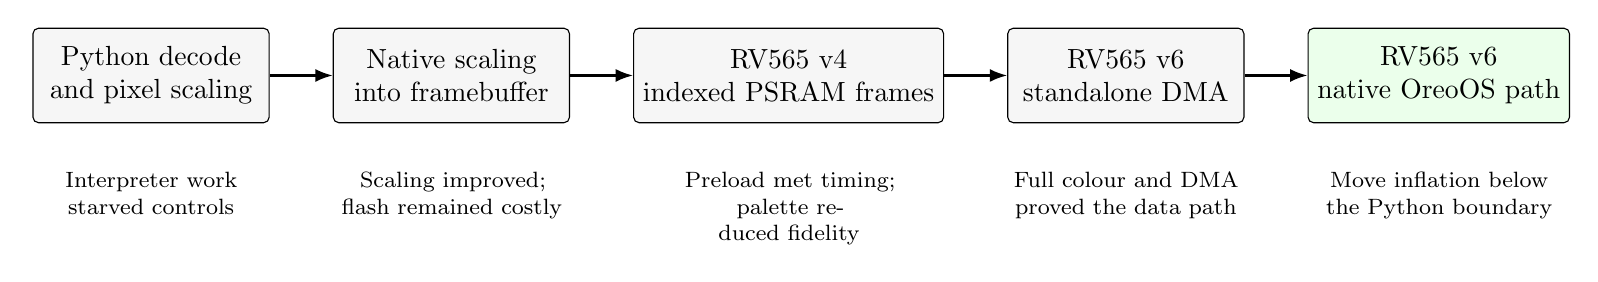
\begin{tikzpicture}[
  stage/.style={draw, rounded corners=2pt, minimum width=30mm,
                minimum height=12mm, align=center, fill=gray!7},
  lesson/.style={font=\footnotesize, align=center, text width=29mm},
  arrow/.style={-{Latex[length=2.2mm]}, thick},
  node distance=8mm
]
  \node[stage] (python) {Python decode\\and pixel scaling};
  \node[stage, right=of python] (native) {Native scaling\\into framebuffer};
  \node[stage, right=of native] (v4) {RV565 v4\\indexed PSRAM frames};
  \node[stage, right=of v4] (standalone) {RV565 v6\\standalone DMA};
  \node[stage, right=of standalone, fill=green!8] (os) {RV565 v6\\native OreoOS path};

  \draw[arrow] (python) -- (native);
  \draw[arrow] (native) -- (v4);
  \draw[arrow] (v4) -- (standalone);
  \draw[arrow] (standalone) -- (os);

  \node[lesson, below=5mm of python] {Interpreter work\\starved controls};
  \node[lesson, below=5mm of native] {Scaling improved;\\flash remained costly};
  \node[lesson, below=5mm of v4] {Preload met timing;\\palette reduced fidelity};
  \node[lesson, below=5mm of standalone] {Full colour and DMA\\proved the data path};
  \node[lesson, below=5mm of os] {Move inflation below\\the Python boundary};
\end{tikzpicture}}
\caption{RV565 evolved by following the bottleneck exposed by each prototype.
The final stage is not a wholesale replacement of OreoOS; it moves only the
deadline-critical media path into firmware.}
\label{fig:evolution}
\end{figure*}

\subsection{Moving pixels out of Python}

The first correction was a native scaler that wrote RGB565 pixels directly
into the display framebuffer.  This removed nested Python loops and restored
much of the frame budget, but it also revealed the next cost: repeatedly
reading frame-sized payloads from the filesystem.  Optimising the computation
had merely exposed the storage path.

RV565 v4 responded by moving expensive colour analysis to the host.  Each
frame carried an adaptive RGB565 palette and an 8-bit index plane.  Gallery
loaded those independent frame blocks into PSRAM incrementally and the native
module expanded them directly into the output framebuffer.  Blocks were used
instead of one monolithic allocation because a long-running UI can have ample
total PSRAM yet lack one sufficiently large contiguous region.  The design was
fast and robust, but a per-frame palette placed an avoidable ceiling on image
fidelity.

\subsection{Separating the hardware limit from the OS cost}

RV565 v6 returned to full-colour RGB565 frames and compressed each one
independently.  To learn whether the hardware could sustain the intended
playback rate, we temporarily removed the operating system and built a
standalone ESP-IDF experiment.  It inflated frames natively, expanded output
through two internal-memory stripes, and transferred those stripes with SPI2
GDMA.  Smooth full-colour playback in that controlled experiment showed that
the display, bus, memory system, and decoder could form a viable pipeline.

Reintroducing the complete OS made the remaining boundary visible.  Gallery
still performed per-frame Deflate work through MicroPython and then entered a
separate native scaling and display path.  Playback improved substantially but
did not reproduce the standalone behaviour.  RV565 therefore became a
firmware facility: Gallery should retain policy and controls, while parsing,
inflation, stripe production, and transfer form one bounded native operation.
This history is central to the method because the final architecture was not
chosen from a catalogue; it was derived by measuring and relocating the
critical path one layer at a time.

\section{Background and Previous Work}

RV565 combines established ideas---display-native pixels, independent
compression, external memory, and DMA-backed transfers---under the constraints
of an interactive MicroPython system.  This section separates those foundations
from the contribution of their integration.  It first considers direct RGB565
playback, then image and video alternatives, the properties inherited from
Deflate, and finally the ESP32-S3 mechanisms used to build the data path.

\subsection{Display-native playback}

Microcontroller video demonstrations have long stored frames in a form close
to the display representation.  Microchip's AN1415, for example, describes
RGB565 video playback from removable storage~\cite{microchip2012video}.  Such
designs minimise device-side transformation but trade storage capacity for
simple execution.  \system{} retains a display-native decoded frame while
compressing each frame independently to reduce storage and input traffic.

\subsection{JPEG, MJPEG, and general media frameworks}

JPEG is a widely deployed still-image coding standard~\cite{wallace1991jpeg},
and concatenated JPEG images form a practical MJPEG video stream.  Espressif's
current multimedia framework supports MJPEG and H.264 playback, demultiplexing,
rendering, seeking, and audio/video synchronisation~\cite{espressif2026player}.
Its published ESP32-S3 path therefore provides an important implementation
baseline rather than an absence of prior video support.  Our focus differs:
the output is fixed to RGB565, frames are independently Deflate-compressed,
and the runtime is designed to coexist with a MicroPython application system.

\subsection{Deflate and independent frames}

Deflate combines LZ77 back-references with Huffman coding
\cite{deutsch1996deflate}; the zlib wrapper specifies framing and integrity
metadata~\cite{deutsch1996zlib}.  Compressing each frame separately resets the
dictionary at every boundary.  This can sacrifice cross-frame compression,
but it bounds corruption, enables direct seeking, and avoids reconstructing a
dependency chain after a dropped or skipped frame.

\subsection{ESP32-S3 memory and display I/O}

The ESP32-S3 combines dual Xtensa LX7 cores with DMA-capable peripherals and
optional external RAM~\cite{espressif2023datasheet}.  ESP-IDF exposes queued
SPI transactions and DMA-backed LCD transfers~\cite{espressif2026spi}.  These
facilities do not themselves create a video architecture: the relevant design
question is how decoded data is partitioned and scheduled so CPU work overlaps
the panel transfer without violating DMA memory constraints.

\section{The \system{} Method}

The method follows the path of a frame from offline preparation to visible LCD
output.  Its organising principle is to move expensive, unconstrained work to
the host while keeping every device-side stage bounded and observable.  The
subsections define the design goals, independence trade-off, memory and DMA
architecture, file contract, validation rules, encoding process, native
pipeline, and the scheduling boundary through which Gallery retains control.

\subsection{Design goals}

The architecture targets four properties: predictable per-frame work,
display-native colour, bounded device memory, and responsive controls.  It
assumes offline access to substantially more compute than is available on the
badge.  Expensive resize and format decisions are therefore moved to the host;
the device performs only parsing, inflation, nearest-neighbour scaling, and
display transfer.

\subsection{Why frame independence}

RV565 v6 makes every compressed payload a complete frame rather than a delta
from an earlier image.  A decoder can therefore start from any indexed frame
with only the global header and that frame's four-byte length prefix.  This
property is useful beyond seeking: looping does not require decoder history, a
missed deadline can be handled by advancing the frame index, and a damaged
payload cannot alter the dictionary used by later frames.  After one linear
scan builds the offset table in $O(N)$ time, lookup is $O(1)$ and requires four
bytes of logical offset data per frame.  Runtime overhead is higher when those
offsets are represented as MicroPython integer objects rather than a packed
native array.

The cost is deliberately paid in storage.  Deflate's dictionary restarts at
every frame, so repeated content across adjacent frames cannot be referenced
and each payload carries its own zlib framing.  Inter-frame codecs generally
compress video more efficiently, but also require reference pictures, more
decoder state, and catch-up decoding after a seek.  RV565 chooses bounded
reconstruction work and local recovery because predictable latency and control
response are more important here than minimum file size.  The evaluation
reports this storage penalty rather than treating independence as free.

\subsection{End-to-end architecture}

Figure~\ref{fig:architecture} shows the complete path.  Large sequential
objects reside in flash or external RAM.  The active decoded frame is reused.
Two small stripe buffers reside in DMA-capable internal memory.  While GDMA
transfers stripe $n$, the CPU scales stripe $n+1$ into the alternate buffer.

\begin{figure*}[t]
\centering
\resizebox{0.98\textwidth}{!}{%
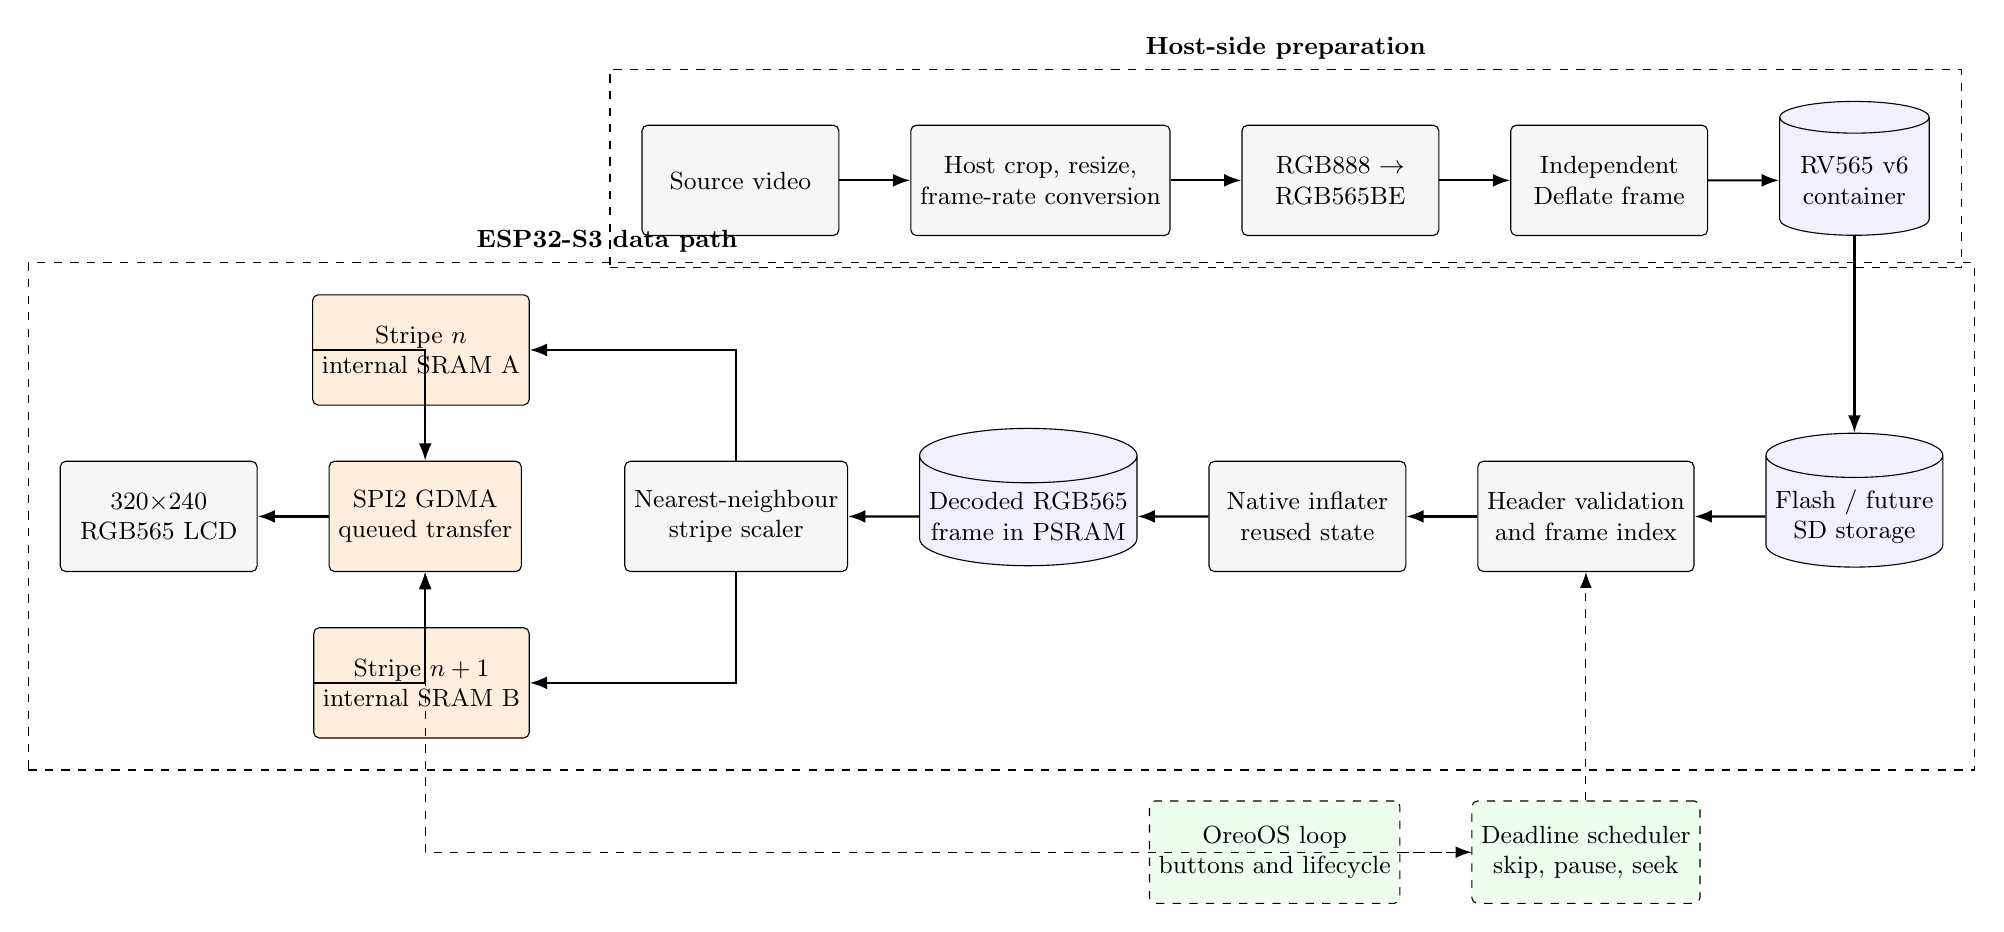
\begin{tikzpicture}[
  font=\small,
  node distance=7mm and 9mm,
  block/.style={draw, rounded corners=2pt, minimum height=14mm,
                minimum width=25mm, align=center, fill=gray!7},
  store/.style={draw, cylinder, shape border rotate=90, aspect=0.25,
                minimum height=17mm, minimum width=19mm, align=center,
                fill=blue!6},
  fast/.style={draw, rounded corners=2pt, minimum height=14mm,
               minimum width=24mm, align=center, fill=orange!13},
  control/.style={draw, dashed, rounded corners=2pt, minimum height=13mm,
                  minimum width=25mm, align=center, fill=green!7},
  flow/.style={-{Latex[length=2.2mm]}, thick},
  ctl/.style={-{Latex[length=2mm]}, dashed}
]
  \node[block] (source) {Source video};
  \node[block, right=of source] (host) {Host crop, resize,\\frame-rate conversion};
  \node[block, right=of host] (rgb) {RGB888 $\rightarrow$\\RGB565BE};
  \node[block, right=of rgb] (deflate) {Independent\\Deflate frame};
  \node[store, right=of deflate] (container) {RV565 v6\\container};

  \node[store, below=25mm of container] (storage) {Flash / future\\SD storage};
  \node[block, left=of storage] (parser) {Header validation\\and frame index};
  \node[block, left=of parser] (inflate) {Native inflater\\reused state};
  \node[store, left=of inflate] (frame) {Decoded RGB565\\frame in PSRAM};
  \node[block, left=of frame] (scale) {Nearest-neighbour\\stripe scaler};
  \node[fast, above left=7mm and 12mm of scale] (stripea)
       {Stripe $n$\\internal SRAM A};
  \node[fast, below left=7mm and 12mm of scale] (stripeb)
       {Stripe $n+1$\\internal SRAM B};
  \node[fast, left=13mm of scale] (dma) {SPI2 GDMA\\queued transfer};
  \node[block, left=of dma] (lcd) {320$\times$240\\RGB565 LCD};

  \node[control, below=29mm of parser] (scheduler) {Deadline scheduler\\skip, pause, seek};
  \node[control, left=of scheduler] (oreo) {OreoOS loop\\buttons and lifecycle};

  \draw[flow] (source) -- (host);
  \draw[flow] (host) -- (rgb);
  \draw[flow] (rgb) -- (deflate);
  \draw[flow] (deflate) -- (container);
  \draw[flow] (container) -- (storage);
  \draw[flow] (storage) -- (parser);
  \draw[flow] (parser) -- (inflate);
  \draw[flow] (inflate) -- (frame);
  \draw[flow] (frame) -- (scale);
  \draw[flow] (scale.north) |- (stripea.east);
  \draw[flow] (scale.south) |- (stripeb.east);
  \draw[flow] (stripea.west) -| (dma.north);
  \draw[flow] (stripeb.west) -| (dma.south);
  \draw[flow] (dma) -- (lcd);
  \draw[ctl] (oreo) -- (scheduler);
  \draw[ctl] (scheduler) -- (parser);
  \draw[ctl] (scheduler.west) -| (dma.south);

  \node[draw, dashed, fit=(source)(host)(rgb)(deflate)(container),
        label=above:{\bfseries Host-side preparation}, inner sep=4mm] {};
  \node[draw, dashed, fit=(storage)(parser)(inflate)(frame)(scale)(stripea)(stripeb)(dma)(lcd),
        label=above left:{\bfseries ESP32-S3 data path}, inner sep=4mm] {};
\end{tikzpicture}}
\caption{The \system{} architecture.  Frame independence permits indexed
seeking and local recovery.  Alternating DMA-capable stripes allow CPU scaling
to overlap display transfer.  Dashed arrows carry scheduling and control.}
\label{fig:architecture}
\end{figure*}

Figure~\ref{fig:hardware-platform} documents the hardware boundary used by the
measurements.  The first panel isolates the LCD clock, data, command/data,
reset, chip-select, power, and backlight paths.  The second places that display
beside the DevKit's flash/PSRAM configuration, USB connection, active-low
controls, and the optional logic-analyser header used for input-latency tests.

\begin{figure*}[!tp]
\centering
\includegraphics[width=0.94\textwidth]{figures/lcd_interface.pdf}
\\[-1mm]\textbf{(a)} LCD connection and signal path
\\[2mm]
\includegraphics[width=0.94\textwidth]{figures/experimental_platform.pdf}
\\[-1mm]\textbf{(b)} Complete experimental circuit
\caption{Board-level schematics of the RV565 test platform.  Panel (a) shows
the 40 MHz write-only ST7789P3 interface.  Panel (b) shows the complete video
and interaction test path; GPIO21 and GPIO33 are reserved for stimulus and
acknowledgement markers in measurement firmware.}
\label{fig:hardware-platform}
\end{figure*}

\subsection{Container format}

An RV565 v6 file begins with a 12-byte header containing a magic identifier,
format version, source width and height, frame rate, flags, and frame count.
Each subsequent frame is stored as a little-endian 32-bit compressed length
followed by one zlib-wrapped Deflate payload.  Successful inflation produces
exactly $w\times h\times2$ bytes in RGB565 big-endian order.  The parser rejects
invalid dimensions, lengths, frame counts, decompressed sizes, and truncated
payloads before presenting a frame.

\begin{table}[t]
\centering
\caption{RV565 v6 file layout. Multi-byte integers are little-endian; decoded
pixels are RGB565 big-endian.}
\label{tab:format}
\resizebox{\columnwidth}{!}{%
\begin{tabular}{rll}
\toprule
Offset & Size & Field \\
\midrule
0 & 3 & Magic, \texttt{RV5} \\
3 & 1 & Version, \texttt{6} \\
4 & 2 & Source width \\
6 & 2 & Source height \\
8 & 1 & Frame rate \\
9 & 1 & Flags \\
10 & 2 & Frame count \\
12 & 4 & Compressed length, frame 0 \\
16 & variable & zlib/Deflate payload, frame 0 \\
$\cdots$ & $\cdots$ & Repeated length and payload \\
\bottomrule
\end{tabular}
}
\end{table}

The length prefix permits a frame-offset table to be constructed in one scan.
Seeking then changes the compressed input position directly and does not
decode preceding frames.  The table requires one offset per frame and can be
built lazily when the first seek occurs.

\subsection{Validation and failure recovery}

Media is checked at two boundaries.  Before transfer, the host ingest tool
decodes every compressed frame and verifies the magic, version, dimensions,
frame rate, frame count, exact RGB565 output length, complete payload coverage,
and absence of trailing data.  It then compares the encoded artifact---not the
source file---with both the media budget and free space reported by the badge.
An interrupted or malformed conversion is consequently rejected before it can
become Gallery input.

Device validation is repeated because stored media cannot be assumed to remain
trusted.  Dimensions must fit the panel, frame rate is limited to 1--30 FPS,
frame count and compressed lengths must be nonzero, and each length must remain
within the file and allocated input buffer.  Inflation succeeds only when it
produces exactly $2wh$ bytes.  The frame index advances only after that check,
so a partial decode is never presented as a new frame.  Gallery currently
fails closed when retrying the frame after rewind also fails.  Independence
would permit a future policy to skip a corrupt indexed payload and resume at
the next valid boundary; that policy is not counted as an implemented result.

\subsection{Host encoding}

The encoder performs aspect-ratio-preserving crop and resize, samples at the
target frame rate, converts to RGB565BE, and compresses every frame separately.
This makes encoder complexity largely irrelevant to device timing.  The
preprocessing step is, however, part of the quality evaluation: resize filter,
source selection, and RGB565 quantisation must be held constant across all
codec baselines.

\subsection{Native decode and stripe pipeline}

The native decoder reuses all large allocations.  It inflates one independent
payload into a decoded frame buffer, then scales output rows into one of two
internal-memory stripes.  The first stripe is queued to SPI GDMA.  While it is
transferred, the CPU fills the other stripe.  A short synchronisation point
precedes reuse of a stripe, after which the roles alternate.  The design does
not assume that external RAM is directly suitable for every DMA transaction.

For a frame deadline $T_f$, measured work is decomposed as

\begin{equation}
\begin{aligned}
T_{frame}={}&T_{read}+T_{inflate}+T_{scale}+T_{lcd}\\
             &-T_{overlap}+T_{os}.
\end{aligned}
\end{equation}

The player meets its target only when the upper tail, not merely the mean, is
below the deadline.  Consequently, the evaluation reports percentile and
worst-observed latency in addition to average throughput.

For each requested frame the firmware follows the same sequence:

\begin{enumerate}
  \item validate the frame index and compressed length;
  \item read the payload into a reused compressed-input buffer;
  \item inflate exactly one RGB565 source frame;
  \item scale the first output stripe into DMA-capable memory;
  \item queue that stripe and prepare the next stripe concurrently;
  \item alternate buffers until the final display row is transferred; and
  \item return timing and status to Gallery before the next OS input poll.
\end{enumerate}

\subsection{OreoOS integration}

Gallery owns playback policy while firmware owns the hot data path.  The
Python layer opens media, requests a frame or seek target, and renders compact
controls.  The native API validates and decodes media and returns structured
status.  At most one frame is advanced per OS tick; accumulated lateness is
discarded instead of triggering a burst of catch-up decodes.  This policy
bounds the time before the next input poll and makes frame dropping preferable
to an unresponsive interface.

\subsection{Scheduling and interaction semantics}

For a clip rate $f$, the period is $P=1/f$ and the nominal deadline of frame
$i$ is

\begin{equation}
d_i=t_0+iP.
\end{equation}

The standalone player advances this absolute deadline after every transfer.
If the clock is more than one period late, it advances both the deadline and
frame index until they again describe a future presentation; late frames are
never decoded merely to catch up.  Gallery applies the same bounded-work rule
at the OS boundary: no more than one frame is decoded during an update tick,
and excess accumulated delay is discarded rather than converted into a burst
of back-to-back work.  Source progress, displayed frames, and dropped frames
are therefore reported separately.

Input preservation and input response are also distinct.  Each active-low
button latches rising and falling GPIO edges in a minimal interrupt handler
while inflation or display transfer is running.  The handler only writes
preallocated bytes; application callbacks remain in the normal OS loop.  A
subsequent poll applies an 8 ms software debounce before emitting one press or
release event.  A short press is thus retained during the native path, but
takes effect only after the current bounded frame operation returns.  Pause
changes playback state, HOME leaves Gallery, and UP/DOWN changes the indexed
seek target.  Input-latency measurement consequently covers the complete
scheduling boundary rather than only GPIO interrupt time.

\section{Evaluation}

Each result is tied to a firmware commit, compiler configuration, test-media
hash, and raw serial log.  This makes a row in the comparison tables traceable
to the code and media that produced it rather than to a manually observed
screen.

\subsection{Platform configuration}

The evaluation platform is an ESP32-S3-DevKitC-1 N16R8 configuration.  Its
module designation provides 16 MiB of flash and 8 MiB of octal PSRAM, while
the application runs on the ESP32-S3's dual Xtensa LX7 cores.  The badge uses
an ST7789-compatible 320$\times$240 panel in RGB565 mode.  OreoOS and Gallery
run under a custom MicroPython v1.28.0 firmware built with ESP-IDF v5.5.1; the
native RV565 module is compiled into that firmware so the compressed-frame hot
path does not cross the Python interpreter for every processing step.

Table~\ref{tab:platform} separates fixed design facts from values that must be
captured for the evaluated build.  This distinction prevents nominal settings
from being mistaken for measured bus, clock, or power behaviour.

\begin{table}[h]
\centering
\caption{Target configuration.}
\label{tab:platform}
\begin{tabular}{@{}p{0.38\columnwidth}p{0.55\columnwidth}@{}}
\toprule
Parameter & Value \\
\midrule
Board & ESP32-S3-DevKitC-1 N16R8 \\
Processor & Dual-core Xtensa LX7 \\
External memory & 16 MiB flash, 8 MiB octal PSRAM \\
Display & ST7789-compatible, 320$\times$240, RGB565 \\
Display interface & 4-wire SPI \\
Operating environment & OreoOS v1.4.119, MicroPython v1.28.0 \\
Firmware framework & ESP-IDF v5.5.1 \\
Encoded source frame & 180$\times$135 RGB565BE \\
Container target & Independent frames at 24 FPS \\
Measured CPU clock & 240 MHz \\
Driver-reported SPI clock & 40 MHz \\
Firmware commit & \wideblank \\
Configuration SHA-256 & \texttt{18a8142f\ldots} \\
Measured supply voltage & \wideblank \\
\bottomrule
\end{tabular}
\end{table}

\subsection{Measurement methodology}

Timing uses the ESP32-S3 monotonic microsecond timer after an initial warm-up.
A frame-work interval begins immediately before payload inflation and ends
when the final queued LCD transaction completes.  Separate timestamps surround
input read, inflation, stripe production, DMA wait, and deferred OS work,
allowing $T_{overlap}$ to be derived rather than guessed.  Displayed FPS is
completed presentations divided by wall time; a drop is a source-frame index
advanced without presentation to restore the absolute schedule.  Reports
include p50, p95, p99, maximum work time, and deadline-miss count.

The completed standalone experiment uses a two-second, 48-frame warm-up and a
30-second, 720-frame timed window.  Ten independently reset runs provide 7,200
frame samples.  Frame percentiles use the pooled empirical distribution;
confidence intervals over run-level aggregates are two-sided 95\% Student-$t$
intervals.  Per-frame records are retained in RAM and printed only after the
timed window, preventing serial output from entering the reported latency.

Control latency is measured from a GPIO edge to entry into the corresponding
Gallery action.  A test-harness GPIO produces the input edge and the
instrumented handler toggles a second line; a logic analyser measures the
interval independently of serial logging.  Pause, seek, and HOME are exercised
at distributed positions within a frame period so presses during inflation and
DMA activity are represented.

Internal SRAM and PSRAM are sampled separately before media open, after
allocation, and during steady-state playback; both current free space and the
minimum-ever watermark are retained.  Energy per displayed frame is the
time-integral of measured supply voltage and current divided by completed
frames.  Raw events, firmware and media hashes, compiler configuration,
warm-up duration, repetition count, and the percentile script accompany each
experiment.  Serial output is disabled during timed windows unless its
overhead is the subject of the test.

\subsection{Workloads and baselines}

The dataset should contain low-motion, high-motion, animation, photographic
noise, dark scenes, hard cuts, and repeated texture.  Clip licences and SHA-256
hashes must be published.  Baselines are raw RGB565, RV565 v4 indexed colour,
RV565 v6 Deflate, and MJPEG configured for comparable output quality.  Where
available, Espressif's player is included as a reference implementation rather
than reimplemented from memory.

\begin{table*}[t]
\centering
\caption{Primary performance comparison.}
\label{tab:results}
\resizebox{\textwidth}{!}{%
\begin{tabular}{lccccccc}
\toprule
Method & Size (MiB) & FPS & Drops & Frame p50 (ms) & p95 (ms) & p99 (ms) & Input p95 (ms) \\
\midrule
Raw RGB565 & \blank & \blank & \blank & \blank & \blank & \blank & \blank \\
RV565 v4 indexed & \blank & \blank & \blank & \blank & \blank & \blank & \blank \\
RV565 v6 Python inflate & \blank & \blank & \blank & \blank & \blank & \blank & \blank \\
RV565 v6 native inflate & \blank & \blank & \blank & \blank & \blank & \blank & \blank \\
RV565 v6 native + DMA stripes & 4.074 & 24.004 & 0 & 38.552 & 39.690 & 40.206 & \blank \\
MJPEG baseline & \blank & \blank & \blank & \blank & \blank & \blank & \blank \\
\bottomrule
\end{tabular}
}
\end{table*}

Table~\ref{tab:results} answers more than whether a clip appears smooth.
Average FPS describes throughput, but dropped frames and upper-tail frame time
show whether the system repeatedly misses its presentation budget.  Input p95
measures the user-visible consequence of those misses: a player that reaches a
high average rate while delaying pause or HOME is not successful inside
OreoOS.  Encoded size is reported beside timing because an architecture that
meets the deadline only by storing raw frames shifts the problem into flash or
external-storage bandwidth.

The comparison must use identical decoded dimensions, frame rate, clip range,
and RGB565 conversion.  MJPEG quality should be selected by a documented
procedure rather than tuned until one preferred result appears.  RV565 v6
Python inflation, native inflation, and native inflation with DMA stripes form
an incremental ablation: the difference between adjacent rows isolates the
cost of the interpreter boundary and then the benefit of overlapping display
transfer.

The completed native-DMA row is the standalone ESP-IDF experiment, not yet the
full OreoOS integration.  All ten runs used the same application, media, and
configuration hashes.  Across 7,200 frames, the maximum observed work time was
40.346 ms, leaving 1.321 ms before the 24 FPS deadline.  Inflation contributed
8.889 ms at p99, while the overlapped LCD path measured 31.321 ms at p99;
scaling and DMA-wait p99 values were 2.608 ms and 28.478 ms, respectively, and
must not be summed because they overlap.  The paced FPS confidence interval is
correspondingly narrow; zero deadline misses and the tail-work margin are the
more informative results.

\begin{table}[h]
\centering
\caption{Resource and energy results.}
\label{tab:resources}
\resizebox{\columnwidth}{!}{%
\begin{tabular}{lccc}
\toprule
Method & SRAM & PSRAM & Energy/frame \\
\midrule
RV565 v6 Python & \blank & \blank & \blank \\
Native framebuffer & \blank & \blank & \blank \\
Native DMA stripes & 79.9 KiB & 0 & \blank \\
\bottomrule
\end{tabular}
}
\end{table}

Table~\ref{tab:resources} complements the timing results with the cost of
achieving them.  Internal SRAM and PSRAM are reported separately because DMA
buffers and general frame storage are not interchangeable on the target.  The
energy-per-frame column prevents a higher-throughput path from hiding a large
power penalty, which matters for a wearable badge.  Together, Tables
\ref{tab:results} and~\ref{tab:resources} describe performance as a resource
envelope rather than as a single headline frame rate.

The standalone SRAM value is incremental internal allocation for decoded-frame
state and two DMA stripes.  It excludes the 23.0 KiB measurement-sample array,
which is identified separately in the raw heap records.  This build does not
allocate PSRAM; the OreoOS-integrated player is evaluated separately because
its framebuffer and interpreter already occupy external memory.

\subsection{Ablation studies}

The evaluation separately disables double buffering, DMA overlap, native
inflation, frame-offset indexing, and real-time OS deferral.  It also compares
flash streaming with external storage and tests playback with radios disabled,
Wi-Fi active, and normal background services active.  The completed native-DMA
experiment is repeated 10 times; confidence intervals use two-sided 95\%
Student-$t$ intervals over run-level aggregates.

Visual quality is measured against the resized RGB888 reference after RGB565
conversion using PSNR and SSIM.  Because Deflate is lossless, RV565 v6's visual
loss arises from spatial resampling and RGB565 quantisation rather than the
compression stage itself.

\section{Discussion and Limitations}

Frame independence exchanges compression efficiency for bounded decoding and
seekability.  The format is currently silent, fixed to RGB565 output, and
designed for small displays.  Deflate decode time remains content-dependent,
so deadline claims must be supported by tail-latency measurements across a
diverse corpus.  Full-screen SPI transfer can remain the dominant cost even
after decode optimisation.  Future work includes SD-backed streaming, audio
output and synchronisation, adaptive quality selection, and evaluation on
other microcontrollers and bus widths.

The implementation should not be compared with H.264 or MJPEG solely on file
size or frame rate.  Those systems offer different quality, compatibility,
hardware support, and feature sets.  The useful comparison is the complete
resource envelope required to provide controllable playback on this specific
class of application platform.

\section{Conclusion}

\system{} treats microcontroller video as an end-to-end scheduling and memory
problem.  Offline display-native conversion, independent compressed frames,
reused decode storage, double-buffered DMA stripes, and deadline-aware OS
integration together form a small and testable architecture.  The standalone
prototype establishes that the hardware path is viable; integrating the same
path beneath Gallery tests the more consequential claim that smooth playback
can coexist with an interactive MicroPython operating system.  More broadly,
the development history shows why isolated decoder optimisation is
insufficient: storage, allocation, colour representation, interpreter
boundaries, scheduling, and display transfer must be treated as one timed
system.

The standalone evaluation sustains 24.004 FPS across 7,200 frames with no
drops or deadline misses and a 40.206 ms pooled p99 frame-work time.  These
results establish the hardware-path claim while deliberately leaving the
OreoOS-integrated and input-latency claims open for their own controlled
measurements.

\section*{Artifact Availability}

The operating system, encoders, standalone benchmark, firmware user modules,
and paper source are available in the OreoOS repository
\cite{bhattacharya2026oreo}.  The final artifact package will additionally
contain firmware hashes, test-media manifests, raw serial logs, analysis
scripts, and exact commands for reproducing every table.

\bibliographystyle{plain}
\bibliography{references}

\end{document}
